\documentclass[12pt]{beamer}
%\documentclass[20pt,handout]{beamer}
\usetheme{Darmstadt}
\usepackage{graphicx}
\usepackage[german]{babel}
\usepackage[T1]{fontenc}
\usepackage[utf8]{inputenc}
\usepackage{tikz}
\setbeamertemplate{footline}[frame number]

\newcommand{\cc}[1]{\includegraphics[height=4mm]{img/#1.png}}
\usepackage{ifthen}
\newcommand{\license}[2][]{\\#2\ifthenelse{\equal{#1}{}}{}{\\\scriptsize\url{#1}}}
\usepackage{textcomp}

\pgfdeclareimage[height=.6cm]{c3d2logo}{./img/c3d2.pdf} 


\pgfdeclarelayer{foreground}
\pgfsetlayers{main,foreground}
\logo{\pgfputat{\pgfxy(-1,0)}{\pgfbox[center,base]{\pgfuseimage{c3d2logo}}}}


\title{Chaos macht Schule}
\author{\small Marius Melzer \& Stephan Thamm\\\large Chaos Computer Club Dresden}
\date{13. Oktober 2012}

\begin{document}
\maketitle

\begin{frame}
  \begin{center}
  \Large Wer sind wir?
  \end{center}
\end{frame}

\section{Motivation}
\subsection{}

\begin{frame}
    \frametitle{Motivation}
    \begin{figure}
        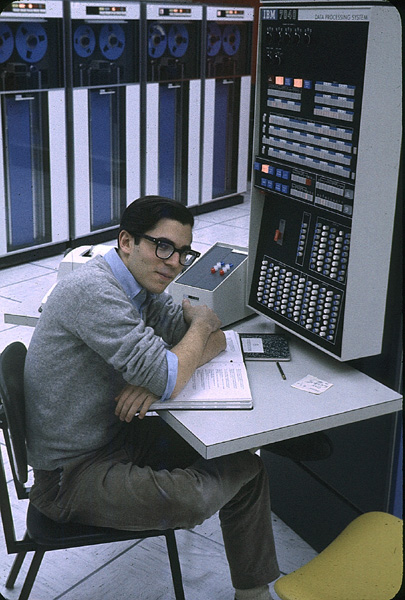
\includegraphics[height=0.7\textheight]{img/computer_alt.jpg}
        \license[http://rchrd.com/weblog/archives/archive\_2005-m03.php]{\cc{by-nc-nd}}
    \end{figure}
\end{frame}

\begin{frame}
    \frametitle{Motivation}
    \begin{figure}
        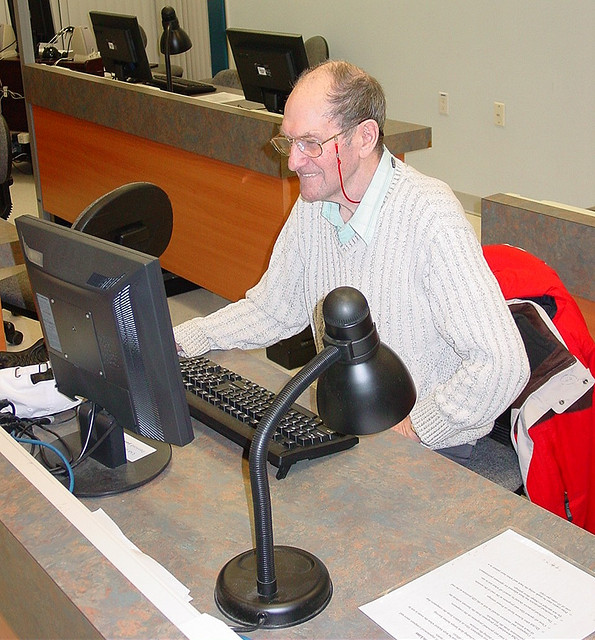
\includegraphics[height=0.7\textheight]{img/computer_senior.jpg}
        \license[http://www.flickr.com/photos/33346162@N07/3113651122/]{\cc{by-nc-nd}}
    \end{figure}
\end{frame}

\begin{frame}
    \frametitle{Motivation}
    \begin{figure}
        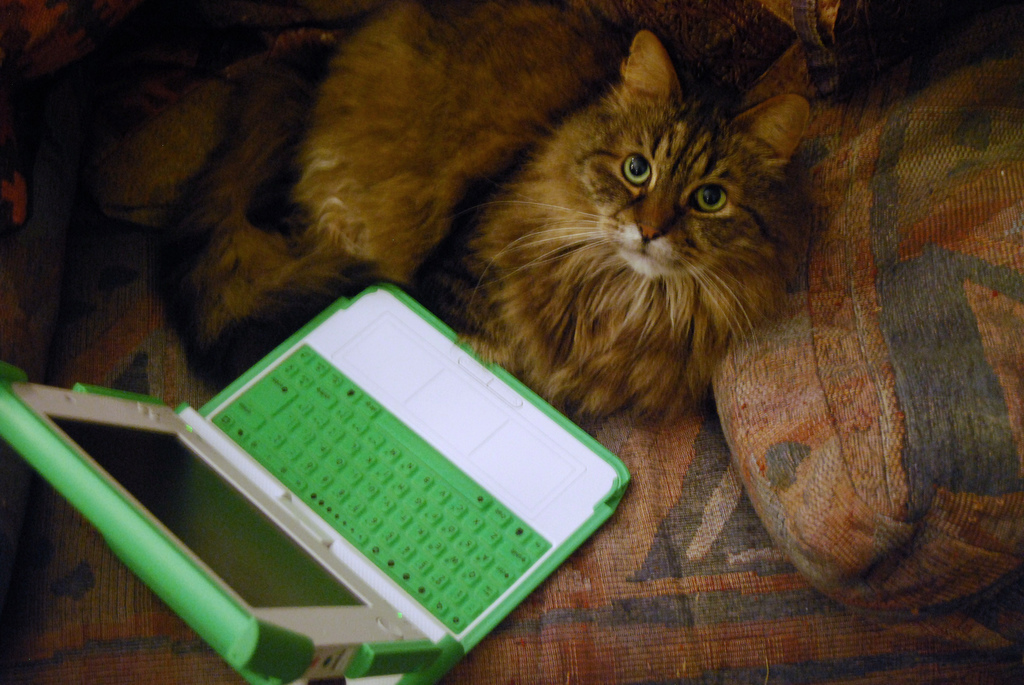
\includegraphics[height=0.7\textheight]{img/computer_katze.jpg}
        \license[http://www.flickr.com/photos/sbisson/2285110239/]{\cc{by-nc-nd}}
    \end{figure}
\end{frame}

\begin{frame}
    \frametitle{Motivation}
    \begin{figure}
        
\includegraphics[height=0.7\textheight]{img/computer_dog.jpg}
        \license[http://www.flickr.com/photos/konszvi/4218539270/]{\cc{by-nc-sa}}
    \end{figure}
\end{frame}

\begin{frame}
    \frametitle{Motivation}
    \begin{figure}
        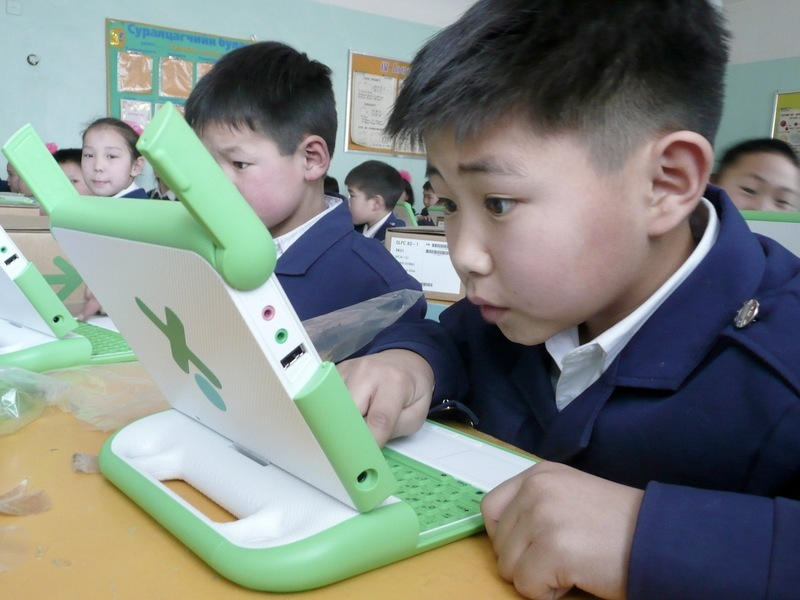
\includegraphics[height=0.7\textheight]{img/computer_olpc.jpg}
        \license[http://www.fotopedia.com/items/flickr-2606362543]{\cc{by}}
    \end{figure}
\end{frame}

\begin{frame}
  \frametitle{Motivation}
  \begin{itemize}
    \item<2-> Jugend wächst mit neuen Medien auf ...
    \item<3-> ... hat nicht automatisch Medienkompetenz
    \item<4-> Von Medienkonsum zu Mediennutzung
    \item<5-> Medienkompetenz vom Bildungssystem nicht erfasst
  \end{itemize}
\end{frame}

\begin{frame}
  \frametitle{Chaos macht Schule}
  \begin{itemize}
    \item<2-> Problem erkannt
    \item<3-> keine Pädagogen ...
    \item<4-> ... aber Kompetenz und Hackerperspektive
    \item<5-> Gründung CmS Gruppen in mehreren Erfas
    \item<6-> in Dresden seit ca. 2 Jahren
  \end{itemize}
\end{frame}

\section{Praxis}
\subsection{}

\begin{frame}
  \frametitle{Schulbesuche}
  \begin{itemize}
    \item<2-> Inhalte
    \begin{itemize}
      \item<3-> Soziale Netzwerke
      \item<4-> Datenschutz
      \item<5-> Internetgrundlagen
    \end{itemize}
    \item<6-> einzelne Stunden (z.B. Gymnasium Bürgerwiese)
    \item<7-> Projekttage (z.B. Ev. Gymnasium Erzgebirge)
    \item<8-> Ganztagsangebot (z.B. Mittelschule Weissig)
  \end{itemize}
\end{frame}

\begin{frame}
  \frametitle{Veranstaltungen für Lehrer}
  \begin{itemize}
    \item<2-> Problembewusstsein schaffen
    \item<3-> Methoden und Lehrmaterialen
    \item<4-> Kontakt herstellen, Austausch
    \item<5-> z.B. Schulinformatiktag
  \end{itemize}
\end{frame}

\begin{frame}
  \frametitle{Elternabende}
  \begin{itemize}
    \item<2-> Panik nehmen
    \item<3-> soziale, nicht technische Probleme
    \item<4-> "'Jugendschutzfilter"'
    \item<5-> "'Cybermobbing"'
  \end{itemize}
\end{frame}

\begin{frame}
  \frametitle{Junghackertrack}
  \begin{itemize}
    \item<2-> Pentabug
    \item<3-> Alarmanlage
    \item<4-> Raketen bauen
    \item<5-> Tastaturlayouts
    \item<6-> Circuit Bending
    \item<7-> Sicherheitsgrundlagen
  \end{itemize}
\end{frame}

\begin{frame}
  \frametitle{Workshops}
  \begin{itemize}
    \item<2-> Datenspuren Freitag
    \begin{itemize}
      \item<2-> Pentabug löten
      \item<2-> Einblick Spiele Programmierung
      \item<2-> Linux installieren
    \end{itemize}
    \item<3-> Teilnehmer des sächs. Informatikwettbewerb
    \begin{itemize}
      \item<3-> Pentabug löten
    \end{itemize}
  \end{itemize}
\end{frame}

\begin{frame}
  \frametitle{Vernetzung}
  \begin{itemize}
    \item<2-> Cross Media Tour
    \begin{itemize}
      \item<3-> verschiedene kostenfreie Medien Workshops
      \item<4-> Zielgruppe: 10-25-Jährige
      \item<5-> Medienkulturzentrum, ColoRadio, TMA Hellerau, riesa efau, ...
      \item<6-> ...und wir
    \end{itemize}
    \item<7-> Medienscouts in Mannheim
    \begin{itemize}
      \item<7-> Zusammenarbeit mit Polizei, Jugendamt, Stadtjugendring
    \end{itemize}
  \end{itemize}
\end{frame}

\section{Inhalte}
\subsection{}

\begin{frame}
  \frametitle{Herangehensweise}
  \begin{itemize}
    \item<2-> Nicht das Internet auf Kinder vorbereiten ...
    \item<3-> ... Kinder auf das Internet vorbereiten
    \item<4-> Kreativer Umgang mit Technik
    \item<5-> Informationelle Selbstbestimmung
    \item<6-> alle Lehrmaterialien frei verfügbar
  \end{itemize}
\end{frame}

\begin{frame}
  \frametitle{Internetgrundlagen}
  \begin{itemize}
    \item Grundlage für Verständnis vieler Probleme
    \item Dezentralität
  \end{itemize}
\end{frame}

\begin{frame}
  \frametitle{Kindernet}
  \begin{figure}
    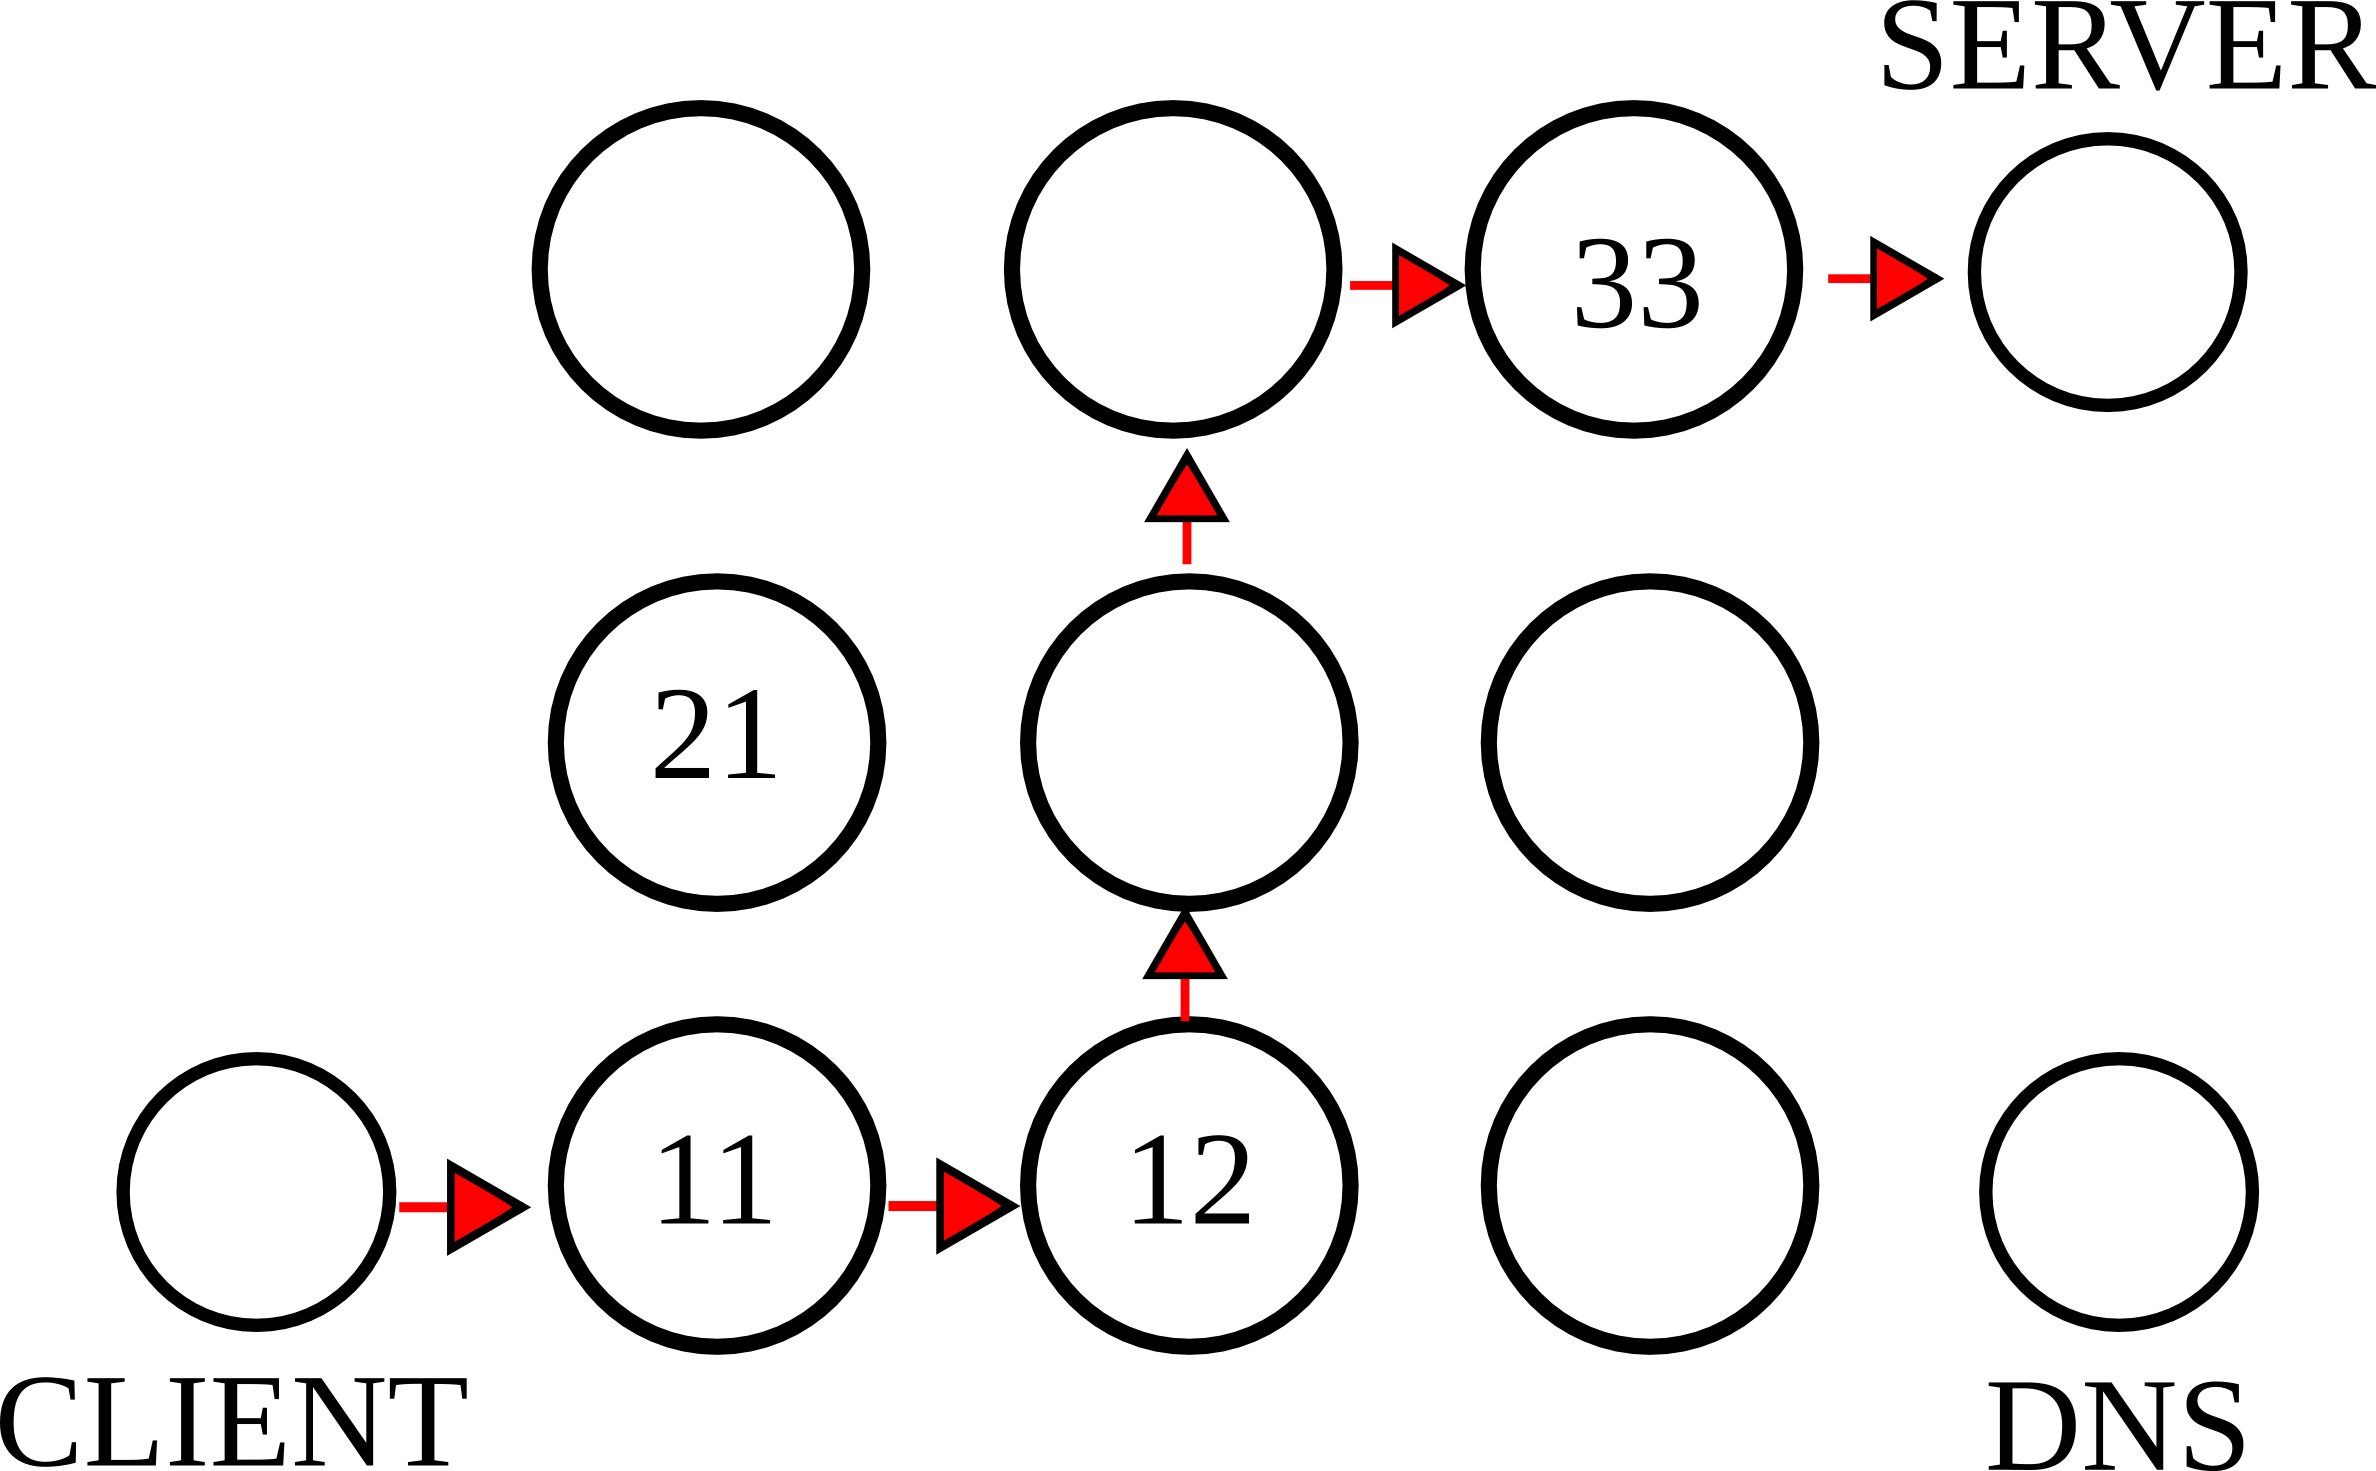
\includegraphics[height=0.7\textheight]{img/kindernet.png}
  \end{figure}
\end{frame}

\begin{frame}
  \frametitle{Datenschutz}
  \begin{figure}
      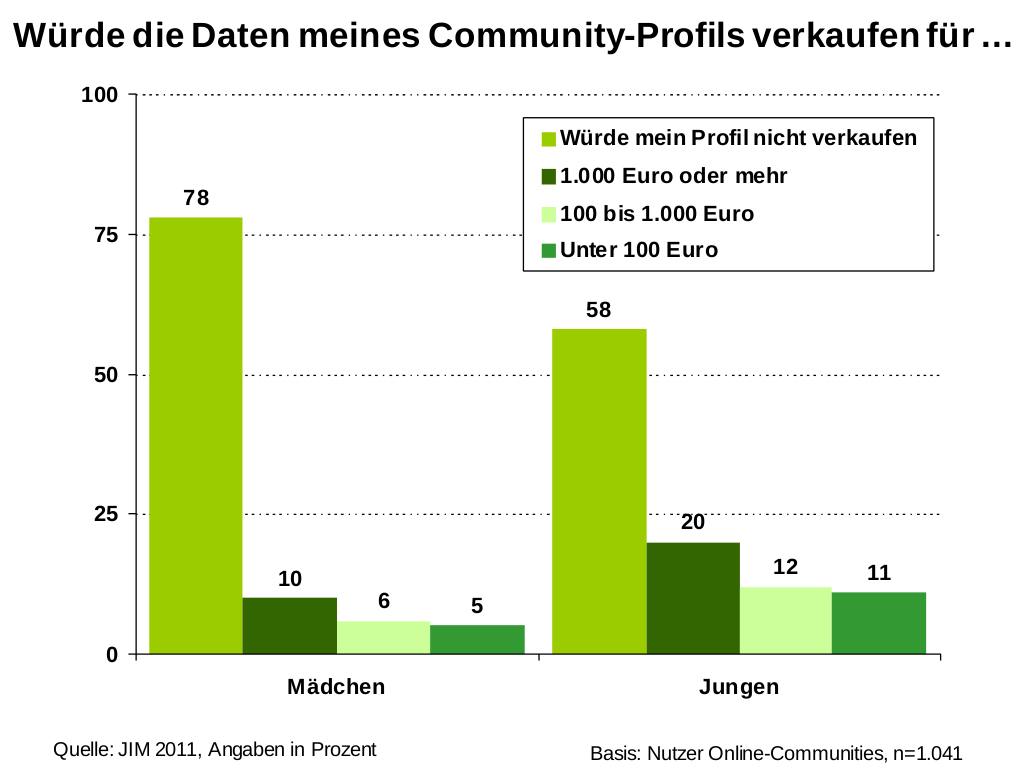
\includegraphics[height=0.7\textheight]{img/jim_verkaufen.png}
      \license[JIM-Studie]{\tiny \copyright Medienpädagogischer Forschungsverbund Südwest (LFK, LMK)}
  \end{figure}
\end{frame}

\begin{frame}
  \frametitle{Datenschutz}
  \begin{itemize}
    \item<2-> Schutz eigener Daten
    \begin{itemize}
      \item<3-> Das Internet vergisst nicht
      \item<4-> Was? Wann? In welchem Kontext? Wem gegenüber?
    \end{itemize}
    \item<5-> Schutz fremder Daten
    \begin{itemize}
      \item<6-> Bilder taggen
      \item<7-> Addressbuchimport
      \item<8-> Selbstbestimmung!
    \end{itemize}
    \item<9-> Kinderbook
  \end{itemize}
\end{frame}

\begin{frame}
  \frametitle{Passwortsicherheit}
  \begin{itemize}
    \item (nCuAj.§Tsm!f
    \item IchLiebeDich
    \item .§)=")=`
    \item 123456
    \item alkmgfksjr
    \item Mks?o/.u,ePsw!
  \end{itemize}
\end{frame}

\begin{frame}
  \frametitle{Soziale Netzwerke}
  \begin{figure}
    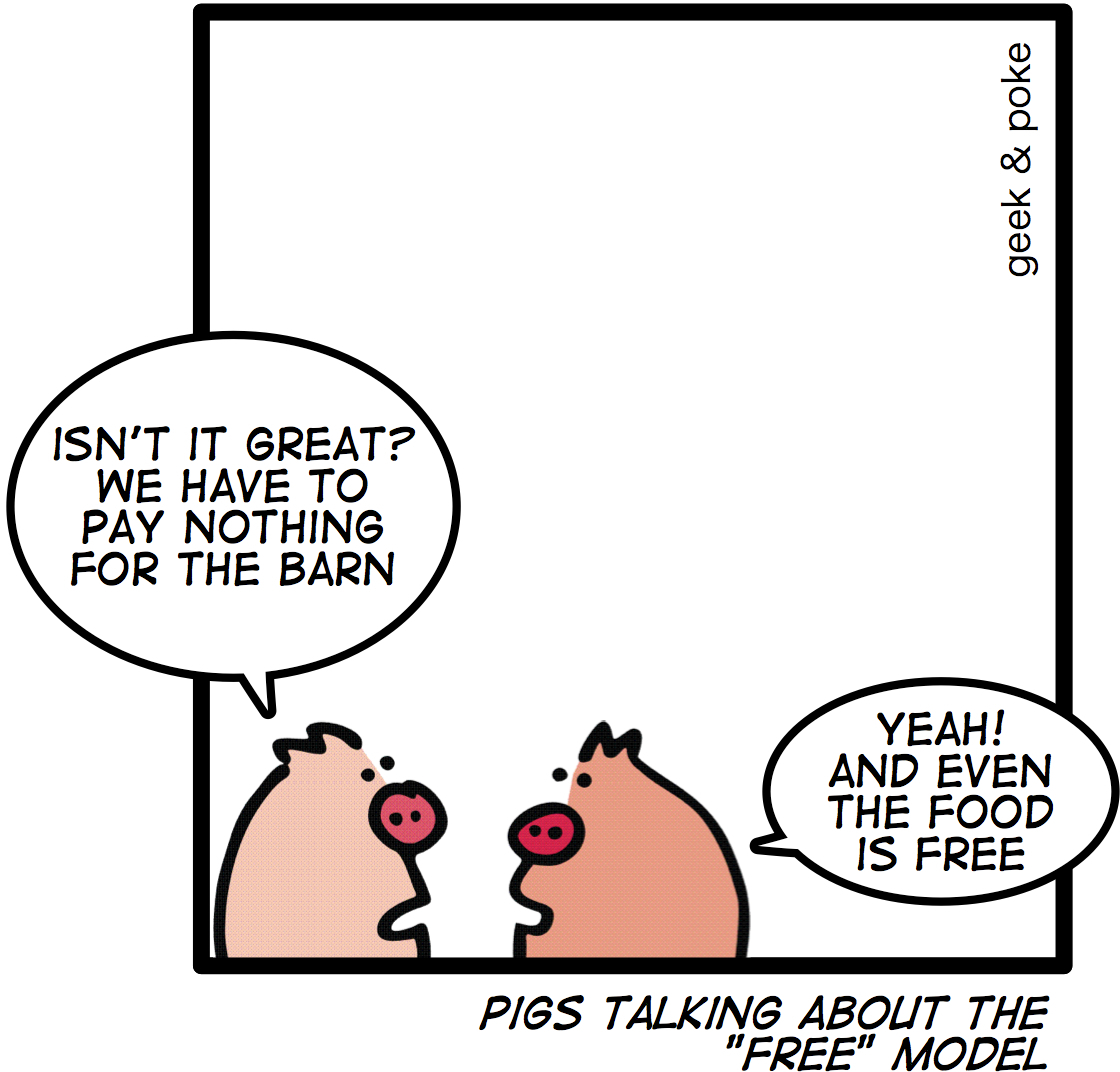
\includegraphics[height=0.7\textheight]{img/business_pigs.jpg}
  \end{figure}
\end{frame}

\begin{frame}
  \frametitle{Soziale Netzwerke}
  \begin{itemize}
    \item<2-> Keine Anleitung zu Facebook-Einstellungen ...
    \item<3-> ... zur Reflexion anregen
    \item<4-> Geschäftsmodelle raten
    \item<5-> Was kann man preisgeben, was lieber nicht?
  \end{itemize}
\end{frame}

\begin{frame}
  \frametitle{Tracking und Selbstschutz im Internet}
  \begin{itemize}
    \item<2-> Verständnis
    \begin{itemize}
      \item Cookies
      \item Zählpixel
      \item Like-Buttons
    \end{itemize}
    \item<3-> Gegenwehr
    \begin{itemize}
      \item Ghostery
      \item Browser-Einstellungen
    \end{itemize}
  \end{itemize}
\end{frame}

\begin{frame}
  \frametitle{Freie Software, freie Lizenzen}
  \begin{itemize}
    \item<2-> Gesellschaftlich sinnvoll
    \item<3-> Ungehinderter Wissensaustausch
    \item<4-> Kreative kooperation
    \item<5-> Nicht auf kommerzielle Produkte prägen
  \end{itemize}
\end{frame}

\begin{frame}
  \frametitle{Löten}
  \begin{itemize}
    \item<2-> Hardware entmystifizieren
    \item<3-> Spaß am Gerät
    \item<4-> Kreativer Umgang mit Technik
  \end{itemize}
\end{frame}

\begin{frame}
  \frametitle{Programmierung}
  \begin{itemize}
    \item<2-> Computer entmystifizieren
    \item<3-> Spaß am Gerät
    \item<4-> Kreativer Umgang mit Technik
  \end{itemize}
\end{frame}

\begin{frame}
  \frametitle{Zum Schluss}
  \begin{itemize}
    \item Sprecht uns an!
    \item Wir kommen auch gern in Ihre Schule
    \item Macht mit!
    \item Fragen? Antworten!
  \end{itemize}
\end{frame}

\end{document}
